\subsection{Hollow Ring/Cylinder}

Consider a hollow, uniform ring of radius $R$ and mass $M$ located in the $X-Y$ plane with its center at the origin rotating about the $Z$-axis as shown in \cref{fig:rotating_ring}.

% !TEX root = ../math_ia.tex
\begin{figure}[H]
  \centering
  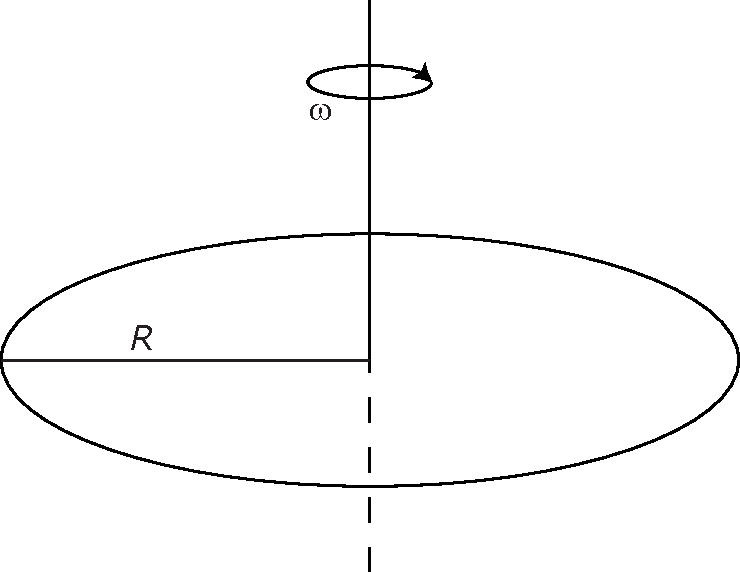
\includegraphics[width=0.25\linewidth]{fig/images/rotating_ring.pdf}
  \caption{A hollow ring rotating about a centered, perpendicular axis with a constant angular velocity $\omega$}
  \label{fig:rotating_ring}
\end{figure}

For this body, all particles are at a constant perpendicular distance from the axis of rotation, thus \cref{eq:total_moment_inertia} can be simplified to the following using the cross-product derivation:
\begin{gather*}
I = \sum_{i=1}^N m_i (|\bm{k}||\bm{r_i}| \sin{\frac{\pi}{2}})^2\\
\end{gather*}

As $\bm{k}$ is a unit vector, its magnitude is $1$ and the magnitude of $\bm{r_i}$ is simply $R$  \begin{gather*}  
I = \sum_{i=1}^N m_i (1 \times R \times 1)^2 \\
I = \sum_{i=1}^N m_i R^2
\end{gather*}

Since the $R^2$ term is constant for all mass particles, the term can be removed from the summation and the inner term is simply summing over the mass of the body:
\begin{align*}
I = R^2\sum_{i=1}^N m_i \\
I = R^2 \times M \\
\end{align*}

Thus, the moment of inertia for a hollow ring has been extrapolated leaving only the overall mass and radius in the formula, as shown in \cref{eq:final_moment_ring}.
\begin{equation}
I_{\text{ring}} = MR^2
\label{eq:final_moment_ring}
\end{equation}

A similar premise can be adopted for a hollow cylinder, with radius $R$ and mass $M$, centered at the origin and rotating around the $Z$-axis as shown in \cref{fig:rotating_hollow_cylinder}.

% !TEX root = ../math_ia.tex
\begin{figure}[H]
  \centering
  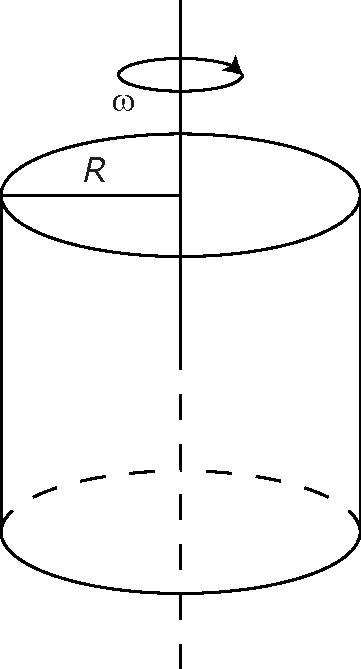
\includegraphics[width=0.25\linewidth]{fig/images/rotating_hollow_cylinder.pdf}
  \caption{A hollow cylinder rotating about a centered, perpendicular axis with a constant angular velocity $\omega$}
  \label{fig:rotating_hollow_cylinder}
\end{figure}

As the perpendicular distance between each point and the axis of rotation is once again a constant $R$, the final result for the moment of inertia will be identical:

\begin{equation}
I_{\text{hollow cylinder}} = MR^2
\label{eq:final_moment_hollow_cylinder}
\end{equation}